\documentclass[journal]{IEEEtran}
\usepackage{cite}
\usepackage{authblk}
\usepackage[pdftex]{graphicx}
\usepackage{amsmath}
\usepackage{algorithmic}
\usepackage{array}
\usepackage{url}

% correct bad hyphenation here
\hyphenation{op-tical net-works semi-conduc-tor}

\begin{document}

% paper title
% For a simple solution, wrap your title in a font size command and enclose it in braces.
% This method may not work as expected because \title may not always respect font size changes directly.
\title{{\Large \textbf{AI in Fintech: Portfolio Formation and Trend Prediction}}}

% author names and affiliations
\author[1]{Qingsen Zhang}
\author[1]{Baiyi Zhang}

% For affiliations, directly adjust the font size using \small, \footnotesize, etc.
\affil[1]{{\small \{zqs, baiyi\}@vt.edu}}
\affil[1]{{\small Department of Computer Science, Virginia Polytechnic Institute and State University, Falls Church, VA, USA}}

% make the title area
\maketitle

% % abstract
\begin{abstract}
This paper presents an AI-driven approach to navigate the complexities of the crypto market. Our approach involves two main tasks: portfolio formation and trend prediction. For portfolio formation, we formulate the selection process as a Constraint Satisfaction Problem (CSP) and solve it using a search algorithm. For trend prediction, we employ Long Short-Term Memory (LSTM) models to predict the future trend of the selected portfolio. Our results, based on the test set spanning from 2019 to 2024, demonstrate the effectiveness of our approach. The LSTM model exhibits robust performance in trend prediction, and the application of these predictions in our investment strategy yields superior outcomes. These results underscore the potential of AI in navigating the complexities of the crypto market and highlight the effectiveness of our two-pronged, AI-driven approach.
\end{abstract}

% % Note that keywords are not normally used for peerreview papers.
% \begin{IEEEkeywords}
% IEEE, journal, \LaTeX, paper, template.
% \end{IEEEkeywords}

\section{Introduction}
% The very first letter is a 2 line initial drop letter followed by the rest of the first word in caps.
\IEEEPARstart{A}{rtificial} intelligence (AI) has been making significant strides in various sectors, and finance is no exception. The application of AI in finance, often referred to as “Fin-Tech,” has been transformative, enabling automation, enhancing decision-making, and revolutionizing customer experiences\cite{bartram2020artificial}. However, one area within the financial sector that is still relatively unexplored in terms of AI application is the cryptocurrency market.

Cryptocurrencies, a relatively new asset class, have gained substantial attention due to their high volatility and potential for significant returns \cite{10356083}. Despite their growing popularity, the application of traditional financial methodologies to this new asset class has been challenging due to its inherent characteristics such as high volatility, 24/7 trading, and lack of regulation. This presents a unique opportunity for the application of AI, which can handle the complexity and unpredictability of the crypto market more effectively than traditional methods \cite{hansun2022multivariate}.

In light of this, our project aims to leverage AI to address two key challenges in the crypto market: portfolio formation and trend prediction. The goal is to develop an AI-driven investment strategy that can navigate the complexities of the crypto market and deliver superior investment outcomes.

Our project design involves two main tasks. The first task is portfolio selection, where we aim to select a subset of over 2000 crypto assets to form a portfolio. This is a combinatorial optimization problem, and we propose to solve it using Constraint Satisfaction Problem (CSP) techniques \cite{gunjan2023brief}. The second task is trend prediction, where we aim to predict the future trend of the selected portfolio. This is a time-series forecasting problem, and we propose to solve it using various AI techniques, including reinforcement learning methods, traditional machine learning algorithms, and deep learning models \cite{zhang2022deep, lim2022dynamic}.

By integrating AI into both the horizontal and vertical interactions of the assets, we aim to maximize the power of AI in investment. Horizontally, AI is used across different assets to identify the optimal combination for the portfolio. Vertically, AI is used to analyze the time-series data of each asset and predict its future trend. This two-pronged approach allows us to harness the full potential of AI in navigating the volatile and unpredictable crypto market.

\section{Methodology}
\subsection{Data Retrieval}
In the course of our research, we employed data derived from Coincap.io, an open-source alternative to CoinMarketCap.com. This platform was chosen due to its extensive data range, allowing for 2000 requests per minute, and its historical depth, which spans up to a decade. Our focus was on the period from 2014 to 2024, a timeframe that encapsulates the lifespan of the majority of cryptocurrencies and includes newly emerged assets. The data acquisition process entailed the retrieval of a comprehensive list of all crypto assets along with their daily price history. Despite the availability of various time intervals, we opted for daily data, as it adequately captures the dynamics of the market. Subsequently, we computed the daily log return, a prevalent financial metric, for each asset. This metric, defined as 
\[
r_t = \ln \left( \frac{P_t}{P_{t-1}} \right)
\]
where $r_t$ represents the log return at time $t$, and $P_t$ and $P_{t-1}$ denote the asset prices at time $t$ and $t-1$ respectively, played a crucial role in our asset selection, trend prediction, and strategy evaluation processes\cite{gupta2024forecasting}.

\subsection{Portfolio Construction}
In the initial stages of our portfolio construction methodology, we established two base cases to provide a comprehensive overview of the crypto market. The first base case was the cumulative return of Bitcoin, the most prominent and widely traded cryptocurrency \cite{chan2002artificial}. The second base case was an equally weighted portfolio of all assets, representing a diversified approach to crypto investment. These base cases served as benchmarks against which the performance of our portfolios was compared.



\begin{figure}[h]
\centering
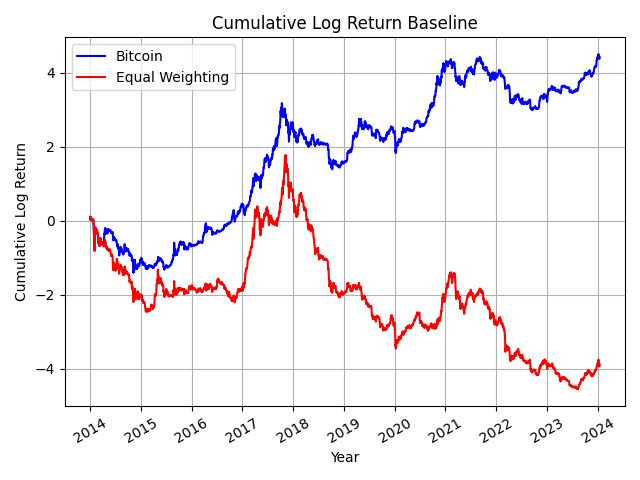
\includegraphics[width=0.5\textwidth]{tex/images/benchmark.png}
\caption{Cumulative Return for Bitcoin and Equally-Weighted Portfolio}
\label{fig:benchmark}
\end{figure}

Figure \ref{fig:benchmark} illustrates the cumulative returns of Bitcoin and the equally weighted portfolio over time. As can be seen, the cumulative return of Bitcoin demonstrated significant growth over the period, despite experiencing two major drops. Notably, after each drop, Bitcoin recovered and continued its upward trajectory. On the other hand, the equally weighted portfolio reached its peak in the last few months of 2017, after which the cumulative return started to decline. It is noteworthy that both Bitcoin and the equally weighted portfolio experienced a drop in 2017, but only Bitcoin managed to recover afterward. These base cases served as benchmarks against which the performance of our portfolios was compared.

The selection process was formulated as a CSP, a robust tool in artificial intelligence for solving combinatorial problems \cite{chen2023deep}. Each asset was treated as a variable, with the domain being the possible states of the asset, specifically its inclusion or exclusion in the portfolio. The constraints were determined by the selection parameters.

A search algorithm was deployed to solve this CSP, exploring the solution space that consisted of all possible combinations of assets. The algorithm began with an empty portfolio and iteratively incorporated assets, ensuring that the inclusion of a new asset did not violate any constraints. The search was guided by a heuristic that favored portfolios with higher expected returns and lower risk, as determined by historical data.

The performance of these portfolios was then evaluated using financial indices, including the Sharpe Ratio, Treynor Ratio, and Jensen’s Alpha. These indices provided a comprehensive assessment of the risk-return trade-off and validated the effectiveness of our portfolio construction methodology.

\subsection{Trend Prediction}
The second component of our methodology pertains to trend prediction. For this task, we elected to utilize Long Short-Term Memory (LSTM) models, a type of recurrent neural network that is well-suited for time-series data due to its ability to capture long-term dependencies \cite{10007138}. The LSTM model is designed with memory cells that allow it to learn and remember patterns over long sequences, making it particularly effective for our task of predicting trends in the highly volatile and dynamic crypto market.

Our objective in trend prediction was not to predict the exact return value for the subsequent day, but rather to forecast the overall trend. This is a crucial distinction as predicting exact return values in such a volatile market can be extremely challenging and prone to errors. On the other hand, predicting the trend (i.e., whether the return would be positive or negative) is more feasible and still highly valuable for informing investment decisions.

To facilitate this, we transformed our problem into a binary classification task. We binarized the daily return into two categories: ‘1’ representing a positive return and ‘-1’ indicating a negative return. This binary representation served as our prediction target, simplifying our problem space and making it more manageable for our LSTM model.

The LSTM model was trained using a comprehensive set of features derived from past performance data. These features encapsulated a range of statistical characteristics that capture different aspects of the asset's historical performance over various time periods. The statistical characteristics included measures of central tendency, dispersion, and correlation, while the time periods spanned short-term to long-term ranges. 

The LSTM model was trained to learn from these historical patterns and predict whether the return on the next day would be positive or negative. This learning process involved adjusting the model's parameters to minimize the difference between the model's predictions and the actual outcomes, using a process known as backpropagation through time. By incorporating a diverse set of features that capture different aspects of the asset performance, the LSTM model was able to effectively learn the underlying patterns in the crypto market and make accurate trend predictions.

To ensure a robust evaluation of our model, we adopted a train-test split approach for our dataset. The training set, comprising data from 2014 to 2019, was used to train the LSTM model. This involved presenting the model with the feature data and the corresponding targets and allowing the model to learn the underlying patterns. The test set, on the other hand, included data from 2019 to 2024. This data was not used during the training process and was used solely to evaluate the model’s predictive performance on unseen data. This approach ensured that our evaluation metrics provided an unbiased estimate of the model's performance when deployed in a real-world setting.

This approach to trend prediction allowed us to harness the power of AI to navigate the inherent volatility and unpredictability of the crypto market. By predicting future trends, we were able to inform our investment decisions and devise effective risk management strategies. This, in turn, enabled us to achieve superior investment outcomes and underscored the potential of AI in revolutionizing the crypto investment landscape.

\section{Result}
 
\begin{figure}[h]
\centering
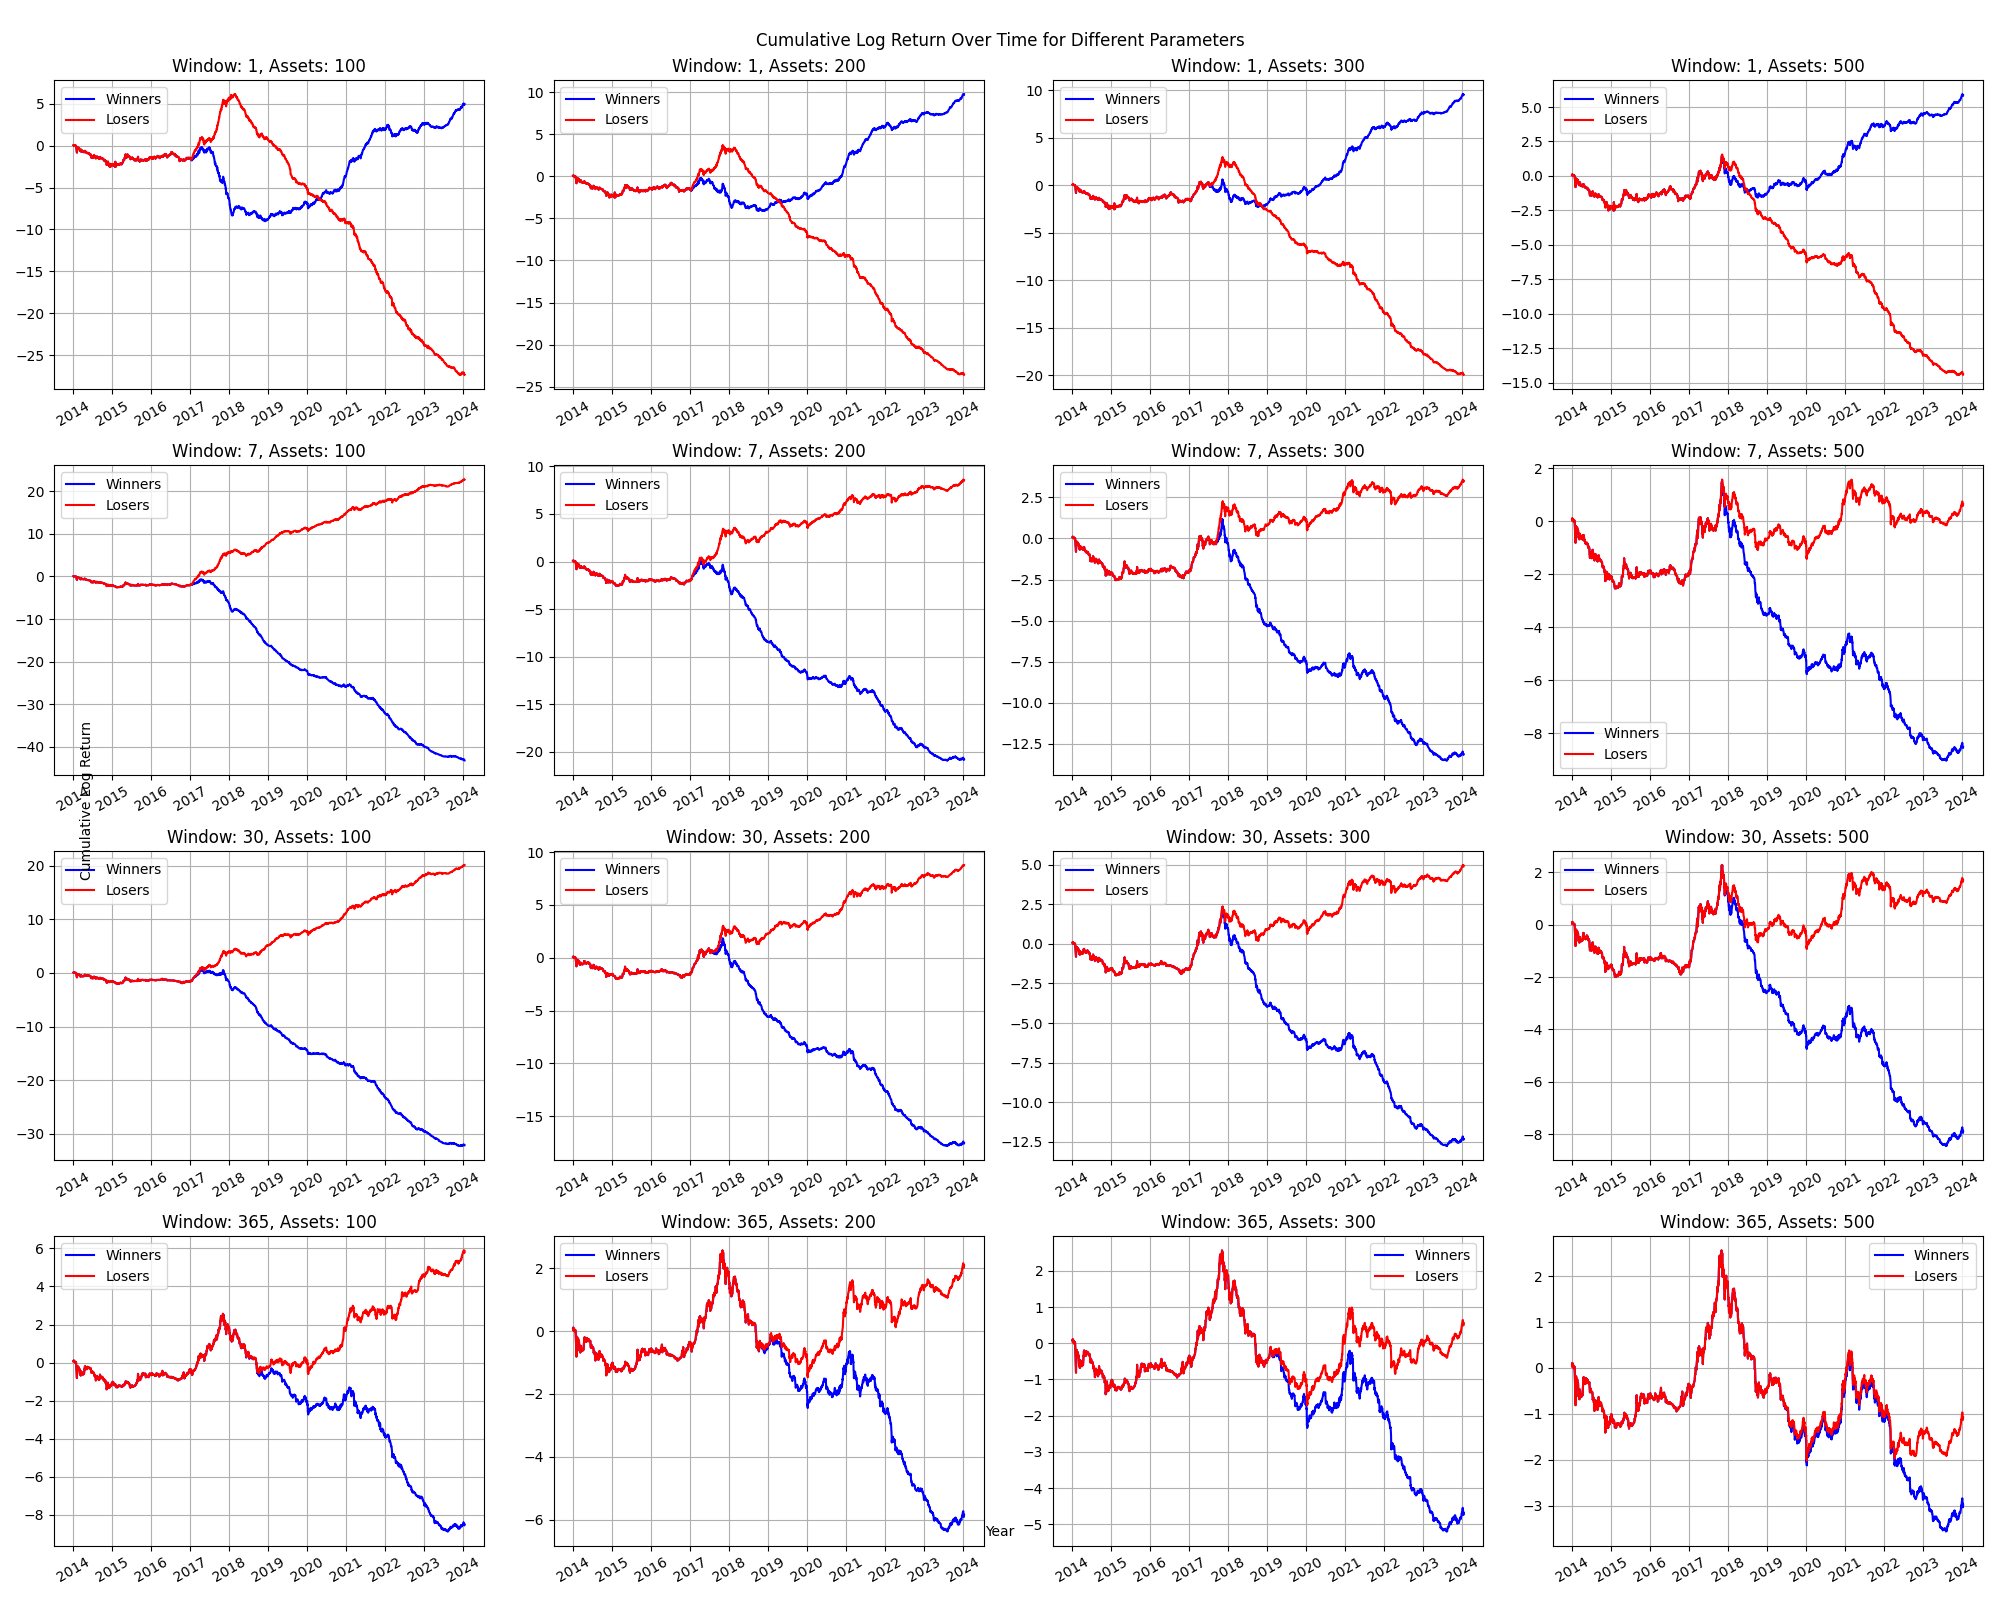
\includegraphics[width=0.5\textwidth]{tex/images/portfolio_matrix.png}
\caption{Portfolio Cumulative Return Matrix}
\label{fig:p_matrix}
\end{figure}
 
\begin{figure}[h]
\centering
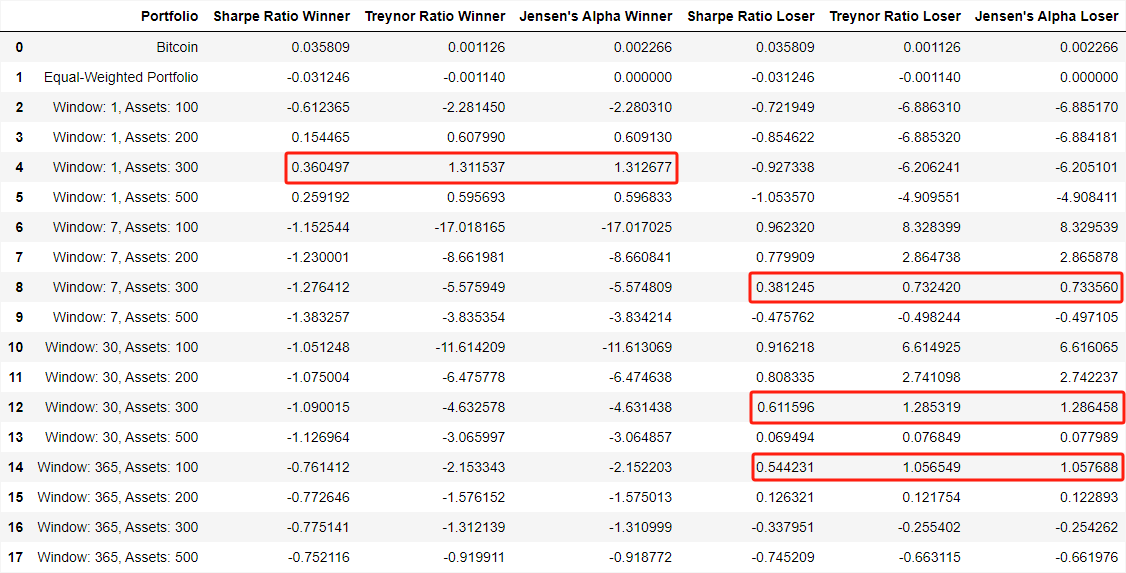
\includegraphics[width=0.5\textwidth]{tex/images/portfolio_index.png}
\caption{Portfolio Financial Index}
\label{fig:p_index}
\end{figure}
\subsection{Portfolio Construction Results}
 Having established the methodology for our project, we now turn our attention to the results derived from our AI-driven approach. This section presents the outcomes of our two-pronged strategy: portfolio formation and trend prediction. We begin with the results of the portfolio formation process, where our AI model was tasked with selecting a subset of over 2000 crypto assets to form an optimal portfolio. Following this, we will present the trend prediction results, based on the portfolio formed in the previous step. This sequential approach allows us to demonstrate the effectiveness of our AI-driven investment strategy in navigating the complexities of the crypto market. 

 In our study, we constructed a total of 32 portfolios, the performance of which is depicted in Figure \ref{fig:p_matrix}. The x-axis represents the number of assets in the portfolio, with values ranging from 100 to 500 assets. The y-axis, the other hand, represents the look-back window, varying from 1 day to 1 week, 1 month, and 1 year.

The performance of the portfolios constructed by past winners is represented in blue, while the portfolios constructed by past losers are represented in red. A key observation from Figure \ref{fig:p_matrix} is that, for the majority of the time, portfolios constructed from past losers tend to yield higher returns in the future compared to those constructed from past winners. This trend, however, does not hold when the asset selection is based solely on the past 1 day’s data, as depicted in the first row of the figure.

Following the initial portfolio formation, we utilized three financial indices to evaluate the performance of all portfolios. This evaluation, illustrated in Figure \ref{fig:p_index}, allowed us to compare each portfolio with our benchmarks. From this comprehensive analysis, we identified four representative portfolios, each corresponding to a different lookback window period category. These portfolios, which are highlighted in Figure \ref{fig:p_index}, were selected based on their superior performance and acceptable risk levels. These selected portfolios will now serve as the foundation for the next phase of our project: trend prediction. In the upcoming sections, we will present the results of applying our AI techniques to these portfolios for predicting future market trends.

\subsection{Trend Prediction Results}


\begin{figure}[h]
\centering
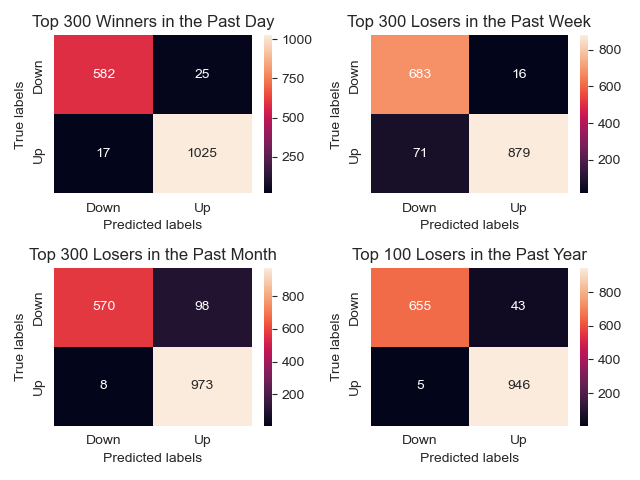
\includegraphics[width=0.5\textwidth]{tex/images/conf-mat.png}
\caption{Confusion Matrices of Strategies}
\label{fig:cof_matrix}
\end{figure}



\begin{table*}[h!]
\centering
\begin{tabular}{|l|c|c|c|c|c|}
\hline
 & \textbf{Accuracy} & \textbf{F-1 Score} & \textbf{Sharpe Ratio} & \textbf{Treynor Ratio} & \textbf{Jensen's Alpha} \\
\hline
\textbf{Bitcoin} & 0.576 & 0.613 & 1.721 & 4.214 & 3.386 \\
\hline
\textbf{Equal-Weighted} & 0.953 & 0.964 & 1.744 & 19.740 & 14.324 \\
\hline
\textbf{Top 300 Winners in the Past Day} & 0.975 & 0.980 & 1.744 & 19.781 & 14.366 \\
\hline
\textbf{Top 300 Losers in the Past Week} & 0.947 & 0.953 & 1.722 & 19.049 & 17.887 \\
\hline
\textbf{Top 300 Losers in the Past Month} & 0.936 & 0.948 & 1.713 & 18.779 & 16.985 \\
\hline
\textbf{Top 100 Losers in the Past Year} & 0.971 & 0.975 & 1.704 & 20.046 & 17.399 \\
\hline
\end{tabular}
\vspace{10pt}
\caption{Scores for Strategies after Trend Prediction}
\label{tab:scores}
\end{table*}


The LSTM model was applied to the four selected portfolios for trend prediction. The results, derived exclusively from the test set spanning from 2019 to 2024, are presented in Figure \ref{fig:cof_matrix}. This figure, a heat map of confusion matrices, provides an intuitive understanding of the model's performance on unseen data. The diagonal elements represent correct predictions, while the off-diagonal elements indicate misclassifications. The high values along the diagonal of the confusion matrices attest to the model's robust ability to learn from past data and accurately predict future trends.

The performance metrics of the LSTM model, including accuracy and F-1 score, are also based solely on the test set and are presented in Table \ref{tab:scores}. These metrics provide a quantitative assessment of the model's predictive performance on unseen data, with high accuracy and F-1 scores indicating its effectiveness in trend prediction.

Upon applying the trend predictions to inform buy-sell decisions, we evaluated the performance of the resulting strategies using financial indices, including the Sharpe Ratio, Treynor Ratio, and Jensen's Alpha. These indices, presented in Table \ref{tab:scores}, are calculated based on the performance of the strategies on the test set. The favorable indices demonstrate the efficacy of our AI-driven investment strategy on unseen data.

In summary, the LSTM model exhibited robust performance in trend prediction on the test set, and the application of these predictions in our investment strategy yielded superior outcomes on unseen data. These results underscore the potential of AI in navigating the complexities of the crypto market and highlight the effectiveness of our two-pronged, AI-driven approach.

\section{Conclusion}
Our study demonstrates the transformative potential of AI in navigating the complexities of the crypto market. By integrating AI into both the horizontal and vertical interactions of the assets, we were able to maximize the power of AI in investment. This integration was manifested in our two-pronged, AI-driven approach, which involved portfolio formation and trend prediction.

In the portfolio formation phase, we utilized a CSP approach to select a subset of over 2000 crypto assets to form an optimal portfolio. This combinatorial optimization problem was solved using a search algorithm guided by a heuristic that favored portfolios with higher expected returns and lower risk. The portfolios formed through this process demonstrated superior performance compared to our base cases, validating the effectiveness of our AI-driven portfolio formation methodology.

In the trend prediction phase, we employed LSTM models, a type of recurrent neural network well-suited for time-series data. The LSTM model was trained to learn from historical patterns in the asset performance data and predict whether the return on the next day would be positive or negative. The model exhibited robust performance in trend prediction, and the application of these predictions in our investment strategy led to impressive results. These results underscore the potential of AI in accurately predicting future trends in the crypto market, thereby informing investment decisions and risk management strategies.

Our two-pronged, AI-driven approach yielded superior outcomes on unseen data, demonstrating the effectiveness of our methodology. The success of our approach highlights the potential of AI in revolutionizing the crypto investment landscape and opens up new possibilities for AI-driven investment strategies.

Looking forward, there are several potential directions for future work. One possibility is to explore other AI techniques for trend prediction, such as Transformer models or Graph Neural Networks, which might capture the dynamics of the crypto market more effectively. These advanced models could potentially improve the accuracy of trend predictions and lead to even better investment outcomes.

Another direction could be to incorporate additional features into the model, such as news sentiment or social media trends. These features could provide valuable insights into market behavior and could enhance the model's ability to predict future trends. Incorporating these additional features would involve collecting and processing large amounts of data, presenting interesting challenges in data management and processing.

Finally, it would be interesting to apply our approach to other financial markets and see if similar results can be achieved. This would involve adapting our methodology to different types of assets and market conditions, providing opportunities to further test and refine our AI-driven investment strategy.

In conclusion, our study demonstrates the potential of AI in navigating the complexities of the crypto market and highlights the effectiveness of our two-pronged, AI-driven approach. We believe that our work contributes to the ongoing efforts to harness the power of AI in finance and opens up new possibilities for future research.

% references section
\bibliographystyle{IEEEtran}
\bibliography{IEEEabrv,tex/proposal/ref}

\end{document}